\documentclass[a4paper]{article}

\usepackage[utf8]{inputenc}

\usepackage{url}
\usepackage[hidelinks]{hyperref}

\usepackage{caption}

\usepackage{listings}

\usepackage{color}

% *** GRAPHICS RELATED PACKAGES ***
%\usepackage[pdftex]{graphicx}
\usepackage{graphicx}
%\usepackage[dvips]{graphicx}
% to place figures on a fixed position
\usepackage{float}

\usepackage[margin=1in]{geometry}

\title{Testing of Network Services}
\author{}
\date{}


\begin{document}

\maketitle

\tableofcontents

\section{Introduction}

The purpose of this lab is to give an insight on system test and to be a teaser to the world of script based automated test execution. During this lab we are going to test LAP-B protocol which is the second layer of the X.25 protocol stack. What makes this lab exotic is that the transmission medium of the protocol is not going to be a physical layer but HTTP instead. The protocol entity to be tested is a web application running on a server : JSON text inside HTTP POST messages can be used for sending LAP-B frames destined for the device under test that will respond with frames in  JSON data in HTTP likewise. As consequence this architecture will give insight on:
\begin{itemize}
  \item script based black-box testing
  \item automated testing of web applications
  \item the application of a generic purpose test execution environment - Ericsson TITAN
  \item TTCN-3 test description language
\end{itemize}

\section{Lab environment}

The software and hardware components that are used during this lab can be seen on Fig.~\ref{fig:lab-arch}.
A virtual machine -- with Ubuntu Linux installed -- is used that contains an Ericsson TITAN test execution environment, a TITAN Eclipse plug-in that is used for creating test scripts and for controlling the execution. As TITAN is a general purpose test execution framework a \emph{test port} has to be used for defining the way of message transmission and reception that are used in the test cases. Since a web server is on the receiving end of the communication the TITAN HTTP port is used for that purpose.

The system under test is LAP-B protocol over HTTP reachable on \url{152.66.246.231:3000}. It is advised to take a look on this page before the measurements and experiment with the protocol operation over the web UI -- without using the JSON API.
Each state of the LAP-B protocol corresponds to a web page and the state transitions can be triggered by sending data through the HTML forms.
This web application uses cookies for storing the state so previously started sessions can be continued until deleting the cookies.

The web application has an additional JSON web service API that is used for verifying the correctness of the protocol's behavior.

The login credentials for the VM (user/pass): \textbf{\emph{ttcn/ttcn}}

\begin{figure}[!htb]
    \centering
    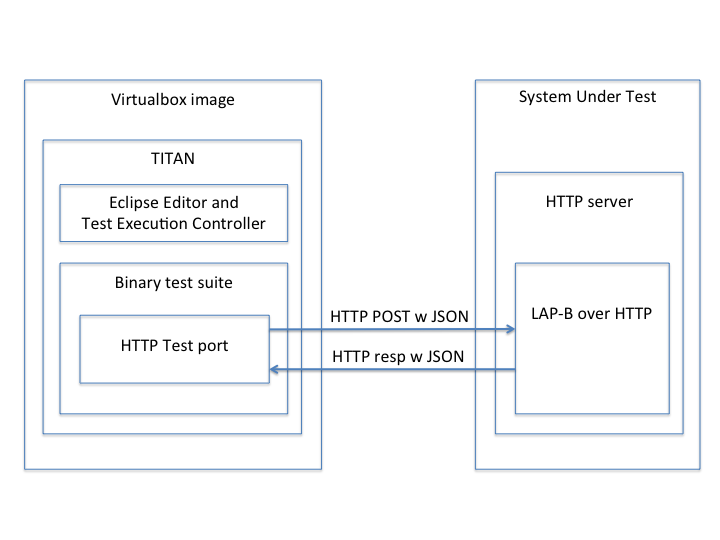
\includegraphics[width=0.9\textwidth]{figures/lab-arch.png}
    \caption{The architecture of the lab}
    \label{fig:lab-arch}
\end{figure}

\section{Testing, protocol testing, web service testing}

\subsection{System test}

The purpose of system test is to make a verdict on the test candidate system in terms of conformance with the functional and non-functional specification. During system test the test candidate is only accessed through its external interfaces -- the internal state is unknown at any time point, it acts like a black box.

When testing the test environment (\emph{tester} in the following) sees the System Under Test (\emph{SUT}) as a black-box. The tester can only send and receive messages from the direction of the SUT through the Point of Control and Observations (PCO). The conformance is verified only through the observable behavior of the SUT over the PCOs.
In a system test the operations declared in the public interface of the system can be executed in an arbitrary sequence with arbitrarily many times therefore the possible sequence and length of an event vector is unbounded/infinite. The result of such unbounded event vector can not be verified therefore a representative selection of them is made what is called \emph{test suite}. The hypothesis is that a thorough test suite guarantees the system's conformance with the specs with high probability.

\subsection{Black-box testing}

In order to execute a test a test suite has to be created. The structure of a test suite is a hierarchy whose basic component is called \emph{test case}. Each test case has a \emph{test purpose} that is basically checking that SUT satisfies one of the criteria of the system specification. Test cases can be further break down into \emph{test steps} that can contain further test steps recursively or \emph{test events}. Test events are considered to be at the lowest level of the hierarchy and to be atomic.
For example a test event can be a reception of a protocol message or sending one, the expiry of a timer etc. The sequence of these atomic test events can be combined into a test step arbitrarily.

The operations executed during a test case run can be split into four phases:
\begin{itemize}
  \item Reset the system. Some protocols have reset message others don't. In that case an appropriate message sequence has to be executed that guarantees to drive the protocol's state machine into the starting state.
  \item Prefix event sequence: the system is driven from the starting state to the state where the goal of the test purpose is verified. This is usually the shortest event sequence denoted by the spanning tree of the system's state machine originated from the starting state.
  \item Execute the operations that verifies the completion of the test case's goal and check whether the system responded appropriately.
  \item We are not done yet at this point! We have to check as a post-condition that the system ended up in the correct state that is checked using a post-condition operations sequence.
\end{itemize}

Telecommunication systems are non-deterministic due to non-error free data transmission and the occurrence of non-deterministic delays over the communication channels. Errors can occur such as data corruption or message loss caused by a bit error in the physical layer or message duplication or reordering of messages because of other reasons. As a consequence beside of the positive outcome a test case must be prepared for handling unexpected events as a result of message sending. All messages sent have to be protected with a timer so that in case of a message loss or deadlock in the SUT it won't not block the tester and the test execution.

The output of the test case execution is the \emph{verdict}. The hypothesis is that if a system responded with the correct output during the 4 phases described above then our terminal state was correct resulting in a \emph{pass} verdict of the test case. If we receive an unexpected message during any message exchange the test case ends in a \emph{fail} verdict also blocking further execution of steps. If the system failed to respond to a request -- that could be caused by network congestion -- it can not be decided whether the operation was correct or not. In such case the verdict is \emph{inconclusive}. There are two more verdicts: \emph{none} when there is no verdict as a result of a test case and \emph{error} where some error occurred during test case execution.


\subsection{Testing of web portals}





\section{Further Reading}

\begin{itemize}
    \item \href{https://qosip.tmit.bme.hu/foswiki/pub/Meres/OpenFlowMScMeresiSegedlet/a19-lantz.pdf}{A Network in a
              Laptop: Rapid Prototyping for Software-Defined Networks}
    \item

          \href{https://qosip.tmit.bme.hu/foswiki/pub/Meres/OpenFlowMScMeresiSegedlet/mininet-hotnets2010-final.pdf}{Presentation
              of conference proceedings on Mininet}
    \item	Mininet page: \url{http://mininet.org/}
    \item	Mininet wiki: \url{https://github.com/mininet/mininet/wiki}
    \item	Mininet introduction: \url{https://github.com/mininet/mininet/wiki/  Introduction-to-Mininet}
    \item	Mininet Python API: \url{http://mininet.org/api/hierarchy.html}
\end{itemize}

\appendix

\section{Entry quiz sample questions}

%\begin{enumerate}

%  \item  Miért nemdeterminisztikus egy távköző rendszer?
%  \item  Milyen ítéletet hozunk, ha a tesztelendő rendszer nem válaszol egy kérésre?
%  \item  Milyen esetekben hozunk inconc ítéletet?
%  \item  Mi az üzenetformátum analógiája webportál esetén?
%  \item  Mi az üzenettípus analógiája webportál esetén?
%  \item  Mi a protokoll állapotátmenet analógiája webportál esetén?
%  \item  Miért van szükség az előfeltételeket beállító eseménysorozatra egy tesztesetben?
%  \item  Milyen válaszokra kell felkészülnük egy tesztesetben egy üzenet kiküldése után?
%  \item  Hogyan kerülhet holtpontra egy rendszer?
%  \item  Mi a tesztvégrehajtás eredménye, ha a teszteset bugot tartalmaz?
%  \item  Mi a kapcsolat a TTCN-3 template-ek és típusok között?
%  \item  Mi a kapcsolat a TTCN-3 template-ek és értékek között?
%  \item  Melyik lehet az alábbi, publikus interfészen deklarált C függvény tesztelését lehetővé tevő TTCN-3 porttípus definíciójának törzse?
%     int f(const char *c)
%        in integer, out charstring
%        out integer, in charstring
%        in integer, inout charstring
%        out integer, inout charstring 
%  \item Definiáljon egy TTCN-3 rekord típust, ami képes egy válasz üzenetet tárolni! (Pontos szintakszis nem elvárt) 
%\end{enumerate}

\section{Lab exercises}

\subsection{Lab environment}

\end{document}